\chapter{Design}\label{ch:design}

This chapter presents our proposed tracking algorithm. Our solution is based on the \gls{deepsort}\cite{Wojke2017_DeepSORT} algorithm, introduced in section \ref{s:sort}. Implementation, especially with respect to efficient use of hardware, has been inspired by \cite{yukai_yang_2020_4294717_fastmot}. 

We use the following notation. \textit{Track} is each unique object of interest (in our case person). Track's \textit{age} is the number of frames it has not been associated with any detection. We will say a track is \textit{active} if its age is below some threshold.  We say track is \textit{confirmed} if it has been associated with a detection at least $n$ times. Track is considered \textit{lost} if it moves out of the frame or is not matched with a detection for $m$ frames.

The algorithm consists of the following high-level steps which are run for each input frame.

% ~ MOT.step
\begin{enumerate}
    \item detect people and faces % detector
    \item extract visual features from detections % feature extractor 
    \item apply Kalman filter % tracker.apply_kalman
    \begin{enumerate}
        \item run prediction for each existing track
        \item mark/remove tracks that move out of frame
    \end{enumerate}
    \item associate existing tracks with detections and update tracks % tracker.update
    \begin{enumerate}
        \item associate \textit{confirmed} tracks based on Mahalanobis distance and visual features 
        \item associate remaining \textit{confirmed} and \textit{active} tracks based on \gls{iou}
        \item associate \textit{unconfirmed} tracks based on \gls{iou}
        \item associate (\gls{reid}) \textit{lost} tracks based on visual features
        \item update tracks % update matched, update not matched (delete/mark_missed/mark_lost)
        \item register new tracks
    \end{enumerate}
    \item extract biometric information from faces
    \item associate faces to tracks
\end{enumerate}


\begin{figure}[htb]
    \newcommand{\mysize}{0.4\textwidth}
     \centering
     \begin{subfigure}[b]{\mysize}
         \centering
         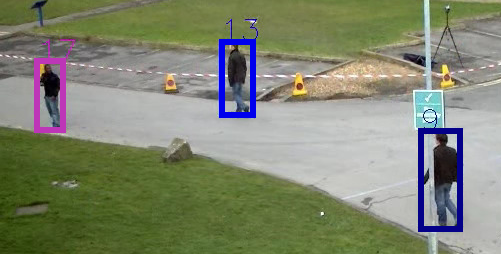
\includegraphics[width=\textwidth]{algo/tracks_at_t0.png}
         \caption{Tracks at time $t$.}
         \label{fig:tracks_at_t0}
     \end{subfigure}
     \hfill
     \begin{subfigure}[b]{\mysize}
         \centering
         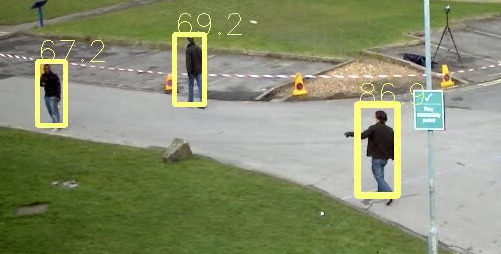
\includegraphics[width=\textwidth]{algo/detections_at_t1.png}
         \caption{Detections at $t + 1$.}
         \label{fig:detections_at_t1}
     \end{subfigure}
     \hfill
     \begin{subfigure}[b]{\mysize}
         \centering
         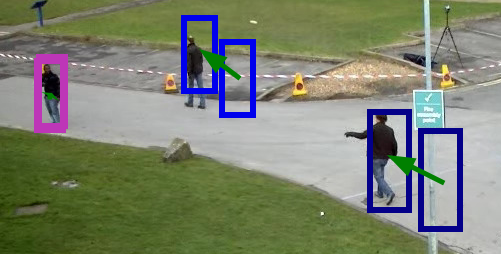
\includegraphics[width=\textwidth]{algo/kalman_predictions_for_t1.png}
         \caption{Kalman predictions for $t + 1$.}
         \label{fig:kalman_predictions_for_t1}
     \end{subfigure}
     \hfill
     \begin{subfigure}[b]{\mysize}
         \centering
         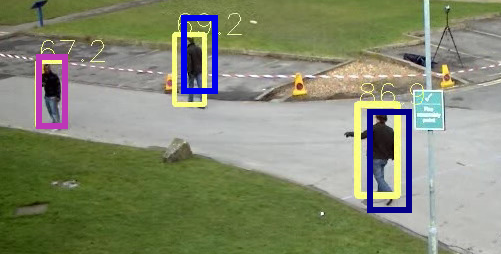
\includegraphics[width=\textwidth]{algo/iou_at_t1.png}
         \caption{Matching is based on \gls{iou} and visual features.}
         \label{fig:matching_at_t1}
     \end{subfigure}
     
    \caption[Visualisation of the main tracking steps.]{Visualisation of the main tracking steps. Images from \cite{MOT16}, modified.}
    \label{fig:simplified_algorithm}
\end{figure}


\section{Detection and Feature Extraction}

\Glspl{cnn}, which were introduced in section \ref{s:cnns}, provide \gls{sota} results for the tasks of detection, feature extraction and age and gender classification. Many \gls{cnn} architectures exist, and the choice of the appropriate one is not obvious. The training dataset selection is also essential.

Our criteria for model selection are accuracy, speed, and, for practical reasons, availability of pre-trained models.

Since performance is a priority, the model should detect both faces and people. Furthermore, we could increase performance if the network used for detection also provided visual features, which would remove the need for a dedicated feature extractor network. \cite{zhang2020fair} proposes such a network while claiming good performance. We found their model to be too slow for real-time processing on our hardware. However, their approach seems very promising, and combining detection and feature extraction might be the best approach in the future.

Comparison of various models is presented in chapter \ref{ch:experiments}.

Based on our analysis, we selected YOLOv4\cite{bochkovskiy2020yolov4} model as the detection model. We use version pre-trained on \cite{shao2018crowdhuman} dataset, with potential fine-tuning on data from the target environment. 

For feature extraction we use \textit{OSnet} architecture from \cite{osnet}, which achieves \gls{sota} results on multiple \gls{reid} datasets and is very lightweight. For details see section \ref{s:reid}. Specifically we use the the version termed \texttt{osnet\_x0\_25} trained on the MSMT17\cite{wei2018person_msmt17} dataset. Pre-trained model is  provided by the paper authors.



\section{Kalman Filter Design}\label{s:kalman_design}

We use the Kalman filter to predict each track's position and update its position after association with a detection. General introduction to Kalman filter is presented in \ref{s:kalman}. This section describes the Kalman model used and its application in our algorithm.

\subsection{Model Design}\label{s:kalman_model_design}

We define the \textit{Kalman state} as a vector
$$
x = ( x_1, y_1, x_2, y_2, \dot{x}_1, \dot{y}_1, \dot{x}_2, \dot{y}_2 ),
$$
where the first four elements represent the coordinates of the top left and bottom right points of the track's bounding box, and the remaining elements are their respective velocities.

Each track is then represented by state means vector $x \in \mathbb{R}^8$ and covariance matrix $P \in \mathbb{R}^{8,8}$. The means vector is initialized from detection with its coordinates and zero velocity. We initialize the covariance matrix as a diagonal matrix. The specific values depend on the observed scene and quality of the detector model.

We assume a constant velocity model for the tracked objects. This assumption is common in literature \cite{Bewley_2016_SORT, Wojke2017_DeepSORT, labbe2014}. Human motion is generally not linear. However, the Kalman filter can reasonably work even when the assumption is not satisfied.

With the constant velocity model in mind, we can define \textit{state transition function} $F$ as
$$
F = \begin{bmatrix}
 1 & 0 & 0 & 0 & 1 & 0 & 0 & 0 \\
 0 & 1 & 0 & 0 & 0 & 1 & 0 & 0 \\
 0 & 0 & 1 & 0 & 0 & 0 & 1 & 0 \\
 0 & 0 & 0 & 1 & 0 & 0 & 0 & 1 \\
 0 & 0 & 0 & 0 & 1 & 0 & 0 & 0 \\
 0 & 0 & 0 & 0 & 0 & 1 & 0 & 0 \\
 0 & 0 & 0 & 0 & 0 & 0 & 1 & 0 \\
 0 & 0 & 0 & 0 & 0 & 0 & 0 & 1 \\
\end{bmatrix}.
$$

Next, we define \textit{measurement function} $H$, which is used to transition from the Kalman state space to a measurement space. In our case, this means moving from an 8-dimensional vector with position and velocity to a 4-dimensional vector with only the position. The measurement function is
$$
H = \begin{bmatrix}
 1 & 0 & 0 & 0 & 0 & 0 & 0 & 0 \\
 0 & 1 & 0 & 0 & 0 & 0 & 0 & 0 \\
 0 & 0 & 1 & 0 & 0 & 0 & 0 & 0 \\
 0 & 0 & 0 & 1 & 0 & 0 & 0 & 0 \\
\end{bmatrix}.
$$

The remaining parts to define are \textit{measurement noise} matrix $R$ and \textit{process noise} matrix $Q$. We define the measurement matrix as a diagonal matrix $R \in \mathbb{R}^{4,4}$ with $\alpha \in \mathbb{R}^+$ on the diagonal. In practice the $\alpha$ value is a hyperpameter based on the precision of the underlying detector model.

We model the process noise as a discrete white noise. Let $\beta \in \mathbb{R}^+$ be a hyperparameter, then the process noise matrix is
$$
Q = \beta \cdot \begin{bmatrix}
 0.25 & 0    & 0    & 0    & 0.5 & 0   & 0   & 0   \\
 0    & 0.25 & 0    & 0    & 0   & 0.5 & 0   & 0   \\
 0    & 0    & 0.25 & 0    & 0   & 0   & 0.5 & 0   \\
 0    & 0    & 0    & 0.25 & 0   & 0   & 0   & 0.5 \\
 0.5  & 0    & 0    & 0    & 1   & 0   & 0   & 0   \\
 0    & 0.5  & 0    & 0    & 0   & 1   & 0   & 0   \\
 0    & 0    & 0.5  & 0    & 0   & 0   & 1   & 0   \\
 0    & 0    & 0    & 0.5  & 0   & 0   & 0   & 1   \\
\end{bmatrix}.
$$

\subsection{Predict and Update}

\textit{Predict} and \textit{update} are the basic steps of the Kalman algorithm. In the prediction part, we try to predict the Kalman state for the next time step.

The update step is based on a measurement $z$. In our algorithm, the measurement is a bounding box of detection associated with the given track. Update consists of computing \textit{residual} $y$ and \textit{Kalman gain} $K$ and then updating the Kalman state. Kalman gain affects how much weight we place on the measurement when combining it with the prediction.

Let $x_t \in \mathbb{R}^8, P_t \in \mathbb{R}^{8,8}$ be the state mean and covariance of the given track at time step $t$. State mean and covariance are separate for each track and time step.

Further, let $F, H, Q, R$ be the various matrices defined in the previous section.

The \textit{predict} step is described by the following equations:
\begin{align}
    \hat{x}_{t+1} &= Fx_t , \\
    \hat{P}_{t+1} &= FPF^T + Q,
\end{align}

and the standard update step is described by:
\begin{align}
    y &= z - H\hat{x}_{t+1} ,\\
    K &= \hat{P}_{t+1} H^T (H \hat{P}_{t+1} H^T + R)^{-1} ,\\
    x_{t+1} &= \hat{x}_{t+1} + Ky ,\\
    P_{t+1} &= (I - KH)\hat{P}_{t+1} .\label{eq:P_update}
\end{align}

We replace equation \ref{eq:P_update} with the following, more numerically stable version from \cite{appliedKalman}:
$$
P_{t+1} = (I - KH)\hat{P}_{t+1}(I - KH)^T + KRK^T.
$$
 
 
% describe how we use it - we run it each frame to predict and then update to smooth detections
\subsection{Application}

We run the Kalman filter on each input frame. First, the \textit{prediction step} is run, and the predicted Kalman state is assigned as a new state to all tracks. This new state is then used for all operations in the algorithm's association step (described in the next section). If the intersection over minimum of the input frame and the track's newly computed bounding box is less than 0.5, the track is considered to have left the scene and is marked as lost.

When using the Mahalanobis distance, both mean and covariance are used for the distance calculation. However, when using \gls{iou} between detections and tracks, only the bounding box information is required. The bounding box information can be extracted easily using the measurement function\footnote{In our case, this simply means taking the first four elements of the state, but in general, the transformation could be more complex.}.

After the detections and tracks are associated, we run the \textit{update step} for each track for which detection was associated. The input measurement is the bounding box of the detection. We also check if the track left the scene same way as in the prediction step.

\section{Track Association}
Associating tracks and detections is a non-trivial task. The tracker has to differentiate between missed detections and objects leaving the scene. It has to decide wherever unmatched detection is a new track or just a false positive.

To make the tracker more robust and accommodate for various errors in underlying models, we perform the matching in multiple steps. We prioritize already established tracks and wait for multiple frames before marking the track as confirmed.

% Why are identity switches bad?
% - because they are hard to detect and fix even if we consider offline postprocessing
% - because they introduce long-term errors, whereas the false positives and false negatives are typically short-term
We find the identity switches as the most relevant and detrimental type of error, because they introduce long-term errors, whereas the false positives and false negatives are typically short-term and do not disrupt the overall trajectory. 

Identity switches can easily happen in groups of multiple people, where the algorithm cannot rely on the position information. Moreover, even relevant visual information can be difficult to obtain due to occlusion. Problematic situations may also be caused by partial or full occlusions from the environment and different visual conditions in various parts of the input frame.

% tady pak už popsat jednotlivý kroky tý asociace
\subsection{Association Steps}

% general
The main part of all association steps is forming a cost matrix for a subset of tracks and a subset of detections. The cost matrix contains the distance between given tracks and detections. Once we have this matrix, we can easily find the minimum cost matching using one of the standard algorithms in polynomial time\cite{kuhn1955hungarian, bourgeois1971extension_munkers}. We start the association with all defections\footnote{By all detections we mean all detections of appropriate class with at least given confidence.}. Detections matched in any step are not used in subsequent steps.

% association - ours vs DeepSort
The first association step is analogical to \gls{deepsort}\cite{Wojke2017_DeepSORT}, which is described in section \ref{s:sort}, with differences described further. The remaining steps are mostly inspired by \cite{yukai_yang_2020_4294717_fastmot}.

% 1st step
In the first step, we associate only \textit{confirmed} tracks. The cost matrix is computed based on Mahalanobis between tracks' states and detections' bounding boxes and feature vectors similarity. Apart from using only the confirmed tracks, another difference from the original \gls{deepsort} is how we store the visual features. The original keeps a gallery of the last $n$ features for each track and computes the distance as a minimum distance between any feature in the gallery and the bounding box feature. 

% 1st step - gallery vs "smooth feature"
Instead of this, we keep only a single feature (vector) for each track. On update, the new feature is calculated as a weighted average of the current and new feature and is normalized afterward. This approach is faster since we need to compute only a single distance for each track. An additional advantage is a potential for robustness. When using the gallery, a single incorrect measurement can take precedence over multiple valid measurements and can remain in the gallery for a long time. 

% 2nd association
In the second step, we associate the \textit{confirmed} tracks which were not associated with any detection in the first step. We also filter out tracks that are not active. The cost matrix is computed based only on \gls{iou} of tracks and detections' bounding boxes.

% 3rd association
The third step associates unconfirmed detections. The cost matrix is computed from \gls{iou} of tracks and detections' bounding boxes, as in the previous step.

% lost tracks re-id
After that, \textit{lost} tracks are associated based only on visual features. This step is similar to the first one; however, no position information is used, as we cannot meaningfully predict the position of lost tracks.

% update matched
Next, we update all matched tracks and set their age to zero. We update their Kalman filter state as described in the previous section.

% cleanup tracks
The next part is dealing with unassociated tracks. We remove those which are unconfirmed, dismissing them as a false positive. We increase the age of remaining unmatched tracks. If the track's age is above some threshold, we mark it as lost.

% register new detections
The last step is creating new tracks from the remaining detections. We initialize each track with a Kalman state as described in section \ref{s:kalman_model_design}.

\section{Age and Gender Classification}

This section describes the age and gender classification of faces and subsequent association with tracks. We introduce optional step for filtering faces based on face alignment. Additionally, we discuss how to produce a final outcome from multiple classification results.

We will be using \glspl{cnn} for the classification task. We find the architectures \textit{GoogLeNet} from \cite{szegedy2015going_googlenet} and \textit{SSRNet} from \cite{yang2018ssr} to be suitable for use in our algorithm. We chose these based on their speed and proclaimed accuracy, as we cannot properly evaluate them due to the dataset problems described in section \ref{s:dataset_age_and_gender}.

\subsection{Face Association}

To propagate the age and gender information to the tracks, we need to associate them with the faces. We calculate a center point for each face's bounding box. We then (for each face) iterate over all tracks and assign the face to the all tracks eligible based on relative bounding box position.

\newcommand{\idkletter}{\xi}
Let $\idkletter_1, \idkletter_2, \idkletter_3, \idkletter_4 \in [0,1]$ be hyperpameters, $c_x, c_y$ the face center, $x, y$ the track's bounding box top left corner coordinates and $w, h$ its width and height. The track is eligible if
$$
x + w \cdot \idkletter_1 \leq c_x \leq x + w \cdot \idkletter_2 \land y + h \cdot \idkletter_3 \leq c_y \leq y  + h \cdot \idkletter_4. 
$$

The main problem with this approach is, we might assign multiple faces to a single track or a single face to multiple tracks. We do not think this issue can be solved without significant overhead. We believe, based on observations from our data, that reasonable choice of the hyperparameters presented above, along with assumed availability of multiple predictions for given tracks, make this issue tolerable.

Another possible approach would be getting better face position approximation from body pose estimation. While this would still leave some cases, where overlap happens (as is inevitable when projecting 3D world to 2D coordinates), it could improve the matching. We did not explore this idea further, as we have found body pose estimation to be too computationally challenging for real-time processing on our hardware.


\subsection{Face Alignment}

As discussed previously, face alignment is critical for explored face classification models. We found that many of the detected faces by selected models are not suitable for further classification. Furthermore, face alignment is a potentially interesting source of information for future expansion, as it allows us to approximate the target's field of view.

The best solution to the classification problems would be to train the model to handle differently aligned faces. However, this can be difficult in practice. Adding alignment-based validation for faces, described in this section, can be seen as a supplementary step. 

One possible approach is to assume that most classifications are correct and solve this when combining multiple predictions. This introduces no additional overhead, as we should always assume that some predictions may be incorrect.

The models typically output a probability for the target classes, which can typically be interpreted as the model's confidence. Another approach might be to consider only detections with very high confidence, assuming that those should be well visible faces. This does not work in practice because models often output extremely high confidence for very low-quality detections, as we have found when experimenting in our dataset.

Facial landmarks localization is topic of \cite{bulat2017far_face_alignment}, where authors present \gls{sota} models for this task. Both 2D and 3D face alignment models are presented. We found the 2D version to be about two times faster while producing good results. The model's output is the location of 68 face landmark points. Visualisation of this output is shown in figure \ref{fig:face_landmark_features}.

Based on these landmarks and some assumptions about human face geometry, we can quickly test if some selected landmarks are approximately at expected locations. We can measure the relative position of the eyes, nose, and mouth and combine this with the face's bounding box size. Based on this, we should be able to classify approximate face position and decide, for example, if the face image is frontal or from the side.

\begin{figure}[htb]
    \centering
    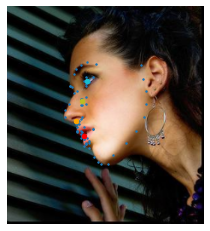
\includegraphics[width=5cm]{face_align_3.png}
    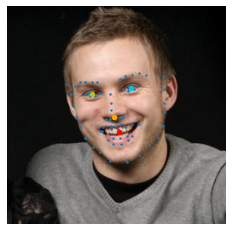
\includegraphics[width=5cm]{face_align_4.png}
    \caption[Visualisation of face landmarks, with certain landmarks highlighted.]{Visualisation of face landmarks, with certain landmarks highlighted. Images are from the  LS3D-W dataset\cite{bulat2017far_face_alignment}.}
    \label{fig:face_landmark_features}
\end{figure}


\subsection{Final Output}

Since we evaluate a video and not a single image, we expect to have multiple predictions for a single track. Some approach is needed to produce a final output of the algorithm. We designed the algorithm to finalize its decision once the track leaves the scene.

% mean, mode, median
Some statistical function is needed to process the multiple predictions into a single outcome. We think reasonable choices are mode for the gender prediction and median for the age prediction.

% 
If the given track has no associated prediction, we output its demographics as ``unknown'', as we have no prior knowledge about the class probabilities. Additionally, it might be reasonable to output ``unknown'' even when there is data present. For example, if there is an equal or almost equal number of predictions for the different gender classes.


\section{Algorithm Hyperparameters}

The presented algorithm has a number of hyperparameters that need to be configured. This section presents their overview and used values in table \ref{table:hyperparameters}. The values are presented mostly for illustrative purposes and as a potential starting point. Target scene, selected models and target goals must be considered when choosing the hyperparameters.

\begin{table}[htb]
    \centering
    
    \begin{tabularx}{\textwidth}{c|X|c}
        name & description & value \\
        \hline
        max\_age & Tracks missed more times are considered lost. & 7  \\
        max\_age\_active & Maximum track's age to be considered active. & 1 \\
        min\_hits & Minimum number of assigned detections to be considered confirmed. & 5 \\
        feature\_alpha & Weight for calculating new visual feature (higher means slower update). & 0.8 \\
        motion\_weight & Weight of the motion distance in contrast to visual feature distance (note that the motion distances are typically about an order larger). & 0.02 \\
        iou\_threshold & Minimal \gls{iou} to consider areas overlaping (when associating with \gls{iou}. & 0.5 \\
        measurement\_noise & Detected bounding box standard deviation. & 100 \\
        process\_noise\_var & Kalman filter process variance. & 10
    \end{tabularx}
    
    \caption{Selected algorithm hyperparameters.}
    \label{table:hyperparameters}
\end{table}

\section{Implementation}

The pipeline is implemented in Python 3.6. We use \textit{TensorRT} framework for optimized \gls{nn} inference on the Jetson platform. \textit{GStreamer} framework along with Jetson-specific NVIDIA plugins is used for efficient video stream processing. \cite{yukai_yang_2020_4294717_fastmot} was used as a basis for developing the pipeline, which proved especially helpful for efficient video processing and using the \textit{TensorRT} framework.

Used Python libraries are \textit{NumPy} for numerical computing and matrix operations, \textit{Pandas} for data manipulation, \textit{FilterPy} for Kalman filter implementation, \textit{py-motmetrics} for \gls{mot} metric calculations and \textit{OpenCV} for video and image processing.

\subsection{Inputs and Outputs}

The system should be usable with various input sources and produce output suitable for additional computer processing.

A standard protocol used in industrial and surveillance cameras is RTSP\cite{schulzrinne1998real_rtsp}. Handling input via this protocol allows the application to be easily connected to live streams from many types of cameras. The application also handles video input from the local filesystem to allow the processing of already recorded videos.

The application outputs location of all confirmed tracks for each frame along with their currently classified demographic information. The final demographic information is stored as a special event when a track leaves the scene. Output for the gender field is either male, female, or ``unknown''. For the age field, the output is either an age range or ``unknown''.

The application can optionally output the average frame rate and proportional time spend in various parts of the algorithms (time spent in detection, association, \dots{}). Additionally, the pipeline can be provided with \textit{ground truth} information for a given file and produce detailed statistics along with overall metrics.

Output can be either send periodically over the network or saved to the local filesystem. Data is saved in the JSON format, which is commonly used for data serialization.